\documentclass[11pt]{scrartcl}

\usepackage[sexy]{evan}
\usepackage{pgfplots}
\pgfplotsset{compat=1.15}
\usepackage{mathrsfs}
\usetikzlibrary{arrows}
\usepackage{graphics}
\usepackage{tikz}
\usepackage{ amssymb }
\usepackage[dvipsnames]{xcolor}
\usepackage[utf8]{inputenc}
\usepackage{longtable}
\usepackage{ragged2e}
\usepackage{listings}
\definecolor{red1}{RGB}{255, 153, 153}
\definecolor{green1}{RGB}{204, 255, 204}
\definecolor{blue1}{RGB}{204, 255, 255}
\definecolor{yellow1}{RGB}{255, 247, 160}

\definecolor{red2}{RGB}{255, 102, 102}
\definecolor{green2}{RGB}{108, 255, 108}
\definecolor{blue2}{RGB}{94, 204, 255}
\definecolor{yellow2}{RGB}{255, 250, 104}

\definecolor{red2.5}{RGB}{255,76,76}
\definecolor{green2.5}{RGB}{54, 247, 54}
\definecolor{blue2.5}{RGB}{51, 189, 255}
\definecolor{yellow2.5}{RGB}{255, 242, 52}


\definecolor{red3}{RGB}{255, 51, 51}
\definecolor{green3}{RGB}{0, 240, 0}
\definecolor{blue3}{RGB}{9, 175, 255}
\definecolor{yellow3}{RGB}{255, 234, 0}

\definecolor{red3.5}{RGB}{229, 25, 25}
\definecolor{green3.5}{RGB}{0, 194, 0}
\definecolor{blue3.5}{RGB}{4, 143, 209}
\definecolor{yellow3.5}{RGB}{255,220,0}

\definecolor{red4}{RGB}{204, 0, 0}
\definecolor{green4}{RGB}{0, 149, 0}
\definecolor{blue4}{RGB}{0, 111, 164}
\definecolor{yellow4}{RGB}{255, 206, 0}


\definecolor{noseve}{RGB}{242,242,242}

\newcommand{\camod}[1]{\frac{\ZZ}{#1 \ZZ}}
\newcommand{\modm}[1]{\text{ mod } #1}
\newcommand{\campm}[1]{\frac{\ZZ}{m\ZZ}}

\usepackage{epigraph}
\renewcommand{\epigraphsize}{\scriptsize}
\renewcommand{\epigraphwidth}{60ex}


\definecolor{dcol0}{HTML}{C8E6C9}
\definecolor{dcol1}{HTML}{D4E9B3}
\definecolor{dcol2}{HTML}{E5ED9A}
\definecolor{dcol3}{HTML}{FFF59D}
\definecolor{dcol4}{HTML}{FFE082}
\definecolor{dcol5}{HTML}{FFCC80}
\definecolor{dcol6}{HTML}{FFAB91}
\definecolor{dcol7}{HTML}{F49890}
\definecolor{dcol8}{HTML}{E57373}
\definecolor{dcol9}{HTML}{D32F2F}

\makeatletter
\newcommand{\getcolorname}[1]{dcol#1}
\makeatother

\newcommand{\dif}[1]{%
    \edef\colorindex{\number\fpeval{floor(#1)}}%
    \edef\fulltext{#1}%
    \colorbox{\getcolorname{\colorindex}}{%
        \ifnum\colorindex>8
            \textbf{\textcolor{white}{\,\fulltext\,}}%
        \else
            \textbf{\textcolor{black}{\,\fulltext\,}}%
        \fi
    }%
}
% Variable para dificultad (inicial 0)
\newcommand{\thmdifficulty}{0}

% Comando para asignar dificultad antes del problema
\newcommand{\problemdiff}[1]{\renewcommand{\thmdifficulty}{#1}}

% Estilo del problema que incluye dificultad antes del título
\declaretheoremstyle[
    headfont=\color{blue!40!black}\normalfont\bfseries,
    headformat={%
      \dif{\thmdifficulty}\quad \NAME~\NUMBER\ifx\relax\EMPTY\relax\else\ \NOTE\fi
    },
    postheadspace=1em,
    spaceabove=8pt,
    spacebelow=8pt,
    bodyfont=\normalfont
]{problemstyle}

    \declaretheorem[style=problemstyle,name=Problema,sibling=theorem]{problema}
    \declaretheorem[style=problemstyle,name=Problema,numbered=no]{problema*}

\usepackage[
backend=biber,
style=alphabetic,
sorting=ynt
]{biblatex}
\addbibresource{referencias.bib}

\title {3.- CSS (Act 3)}
\subtitle{Programación WEB I \\ Centro de Enseñanza Tecnica Industrial}
\date{27 de Agosto de 2025}
\author{Emmanuel Buenrostro 22300891 7F1}


\begin{document}

\maketitle


\begin{center}
   
\includegraphics[scale=0.15]{../cetilogo.jpg} 
\end{center}
\newpage
\tableofcontents


\section{Resumen}

CSS es un lenguaje de estilos utilizado para darle estilo a los documentos HTML. \\
Este se hace mediante distintas etiquetas que le dan valores a los atributos, mediante tres formas distintas de incluirlo en el HTML.

\section{Desarrollo}

\subsection{¿Qué es CSS?}

CSS viene de \textit{Cascading Style Sheets} es el lenguaje de estilos 
utilizado para describir la presentación de documentos HTML.  \\

CSS describe como debe ser renderizado los elementos en la pantalla. \\ 

Es un lenguaje de cascada, porque puede un atributo puede tener varios valores pero solo toma el mas "interno" al elemento. \\

La estructura de CSS consiste de un selector y corchetes, dentro de cada corchete vienen las instrucciones separadas por un ;, cada una viene con una propiedad dos puntos y un valor especifico.  \\
Ejemplo:
\begin{center}
    h1 $\{$color:blue; font-size:12px;$\}$
\end{center}


Para integrarlo dentro de un html puedes incluirlo en un archivo separado y ponerlo en el head:
\begin{lstlisting}
<head>
<link rel="stylesheet" href="stylesheet.css">
</head>
\end{lstlisting}


O de forma interna:
\begin{lstlisting}
<head>
<style>
h1 {color:blue; font-size:12px;}
</style>
</head>
\end{lstlisting}

O inline:

\begin{lstlisting}
    <h1 style="color:blue; font-size:12px;"> Esto es un encabezado </h1>
\end{lstlisting}


\subsection{Ejemplos}

\textbf{Ejemplos del 1-5: Inline, con 5 atributos } \\

\lstinputlisting[language=html]{cssinlineex.html}

\begin{center}
    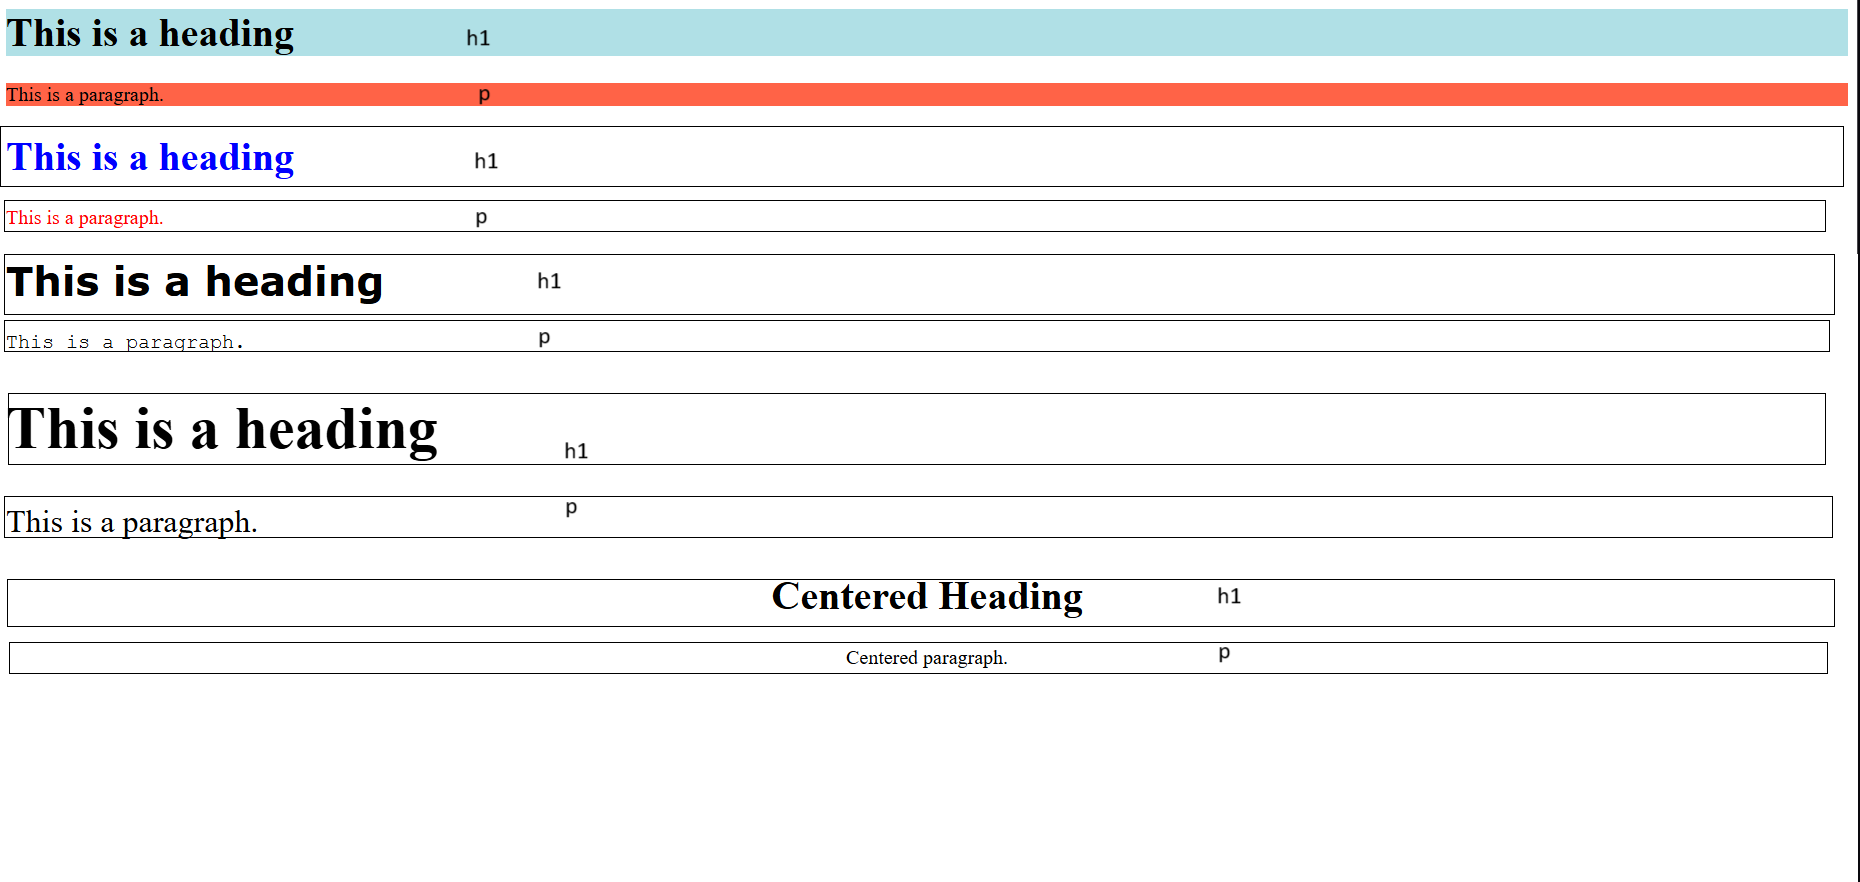
\includegraphics[scale=0.4]{Ex1.png}
\end{center}


\textbf{Ejemplo 6: Internal}
\lstinputlisting[language=html]{cssinternalex.html}

\begin{center}
    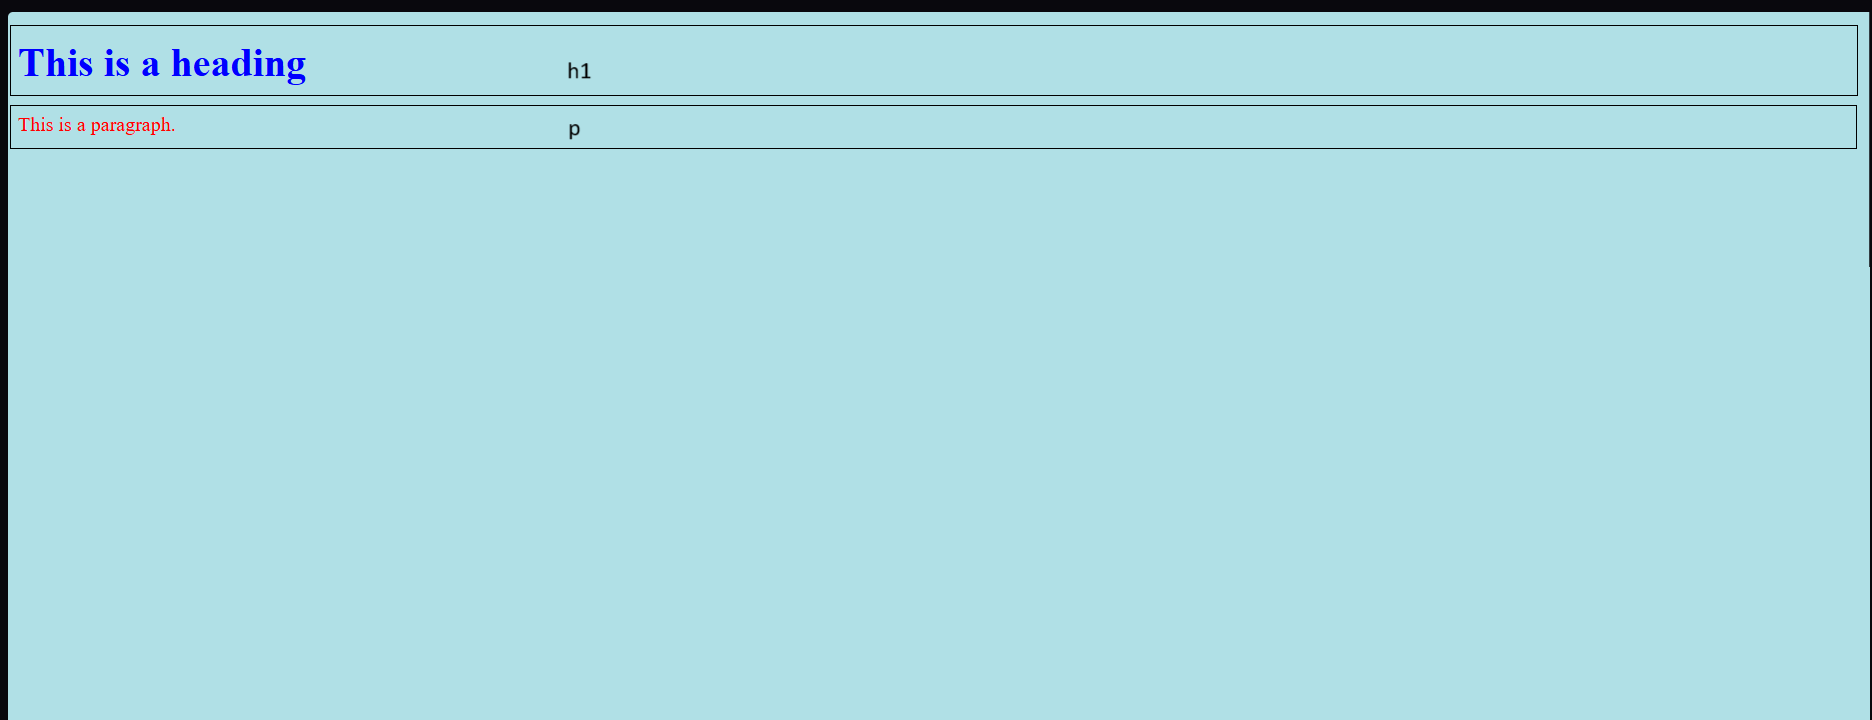
\includegraphics[scale=0.4]{Ex6.png}
\end{center}



\textbf{Ejemplo 7: External} \\

HTML:

\lstinputlisting[language=html]{cssexternalex.html}


CSS:
\lstinputlisting{cssexternalstyles.css}


\begin{center}
    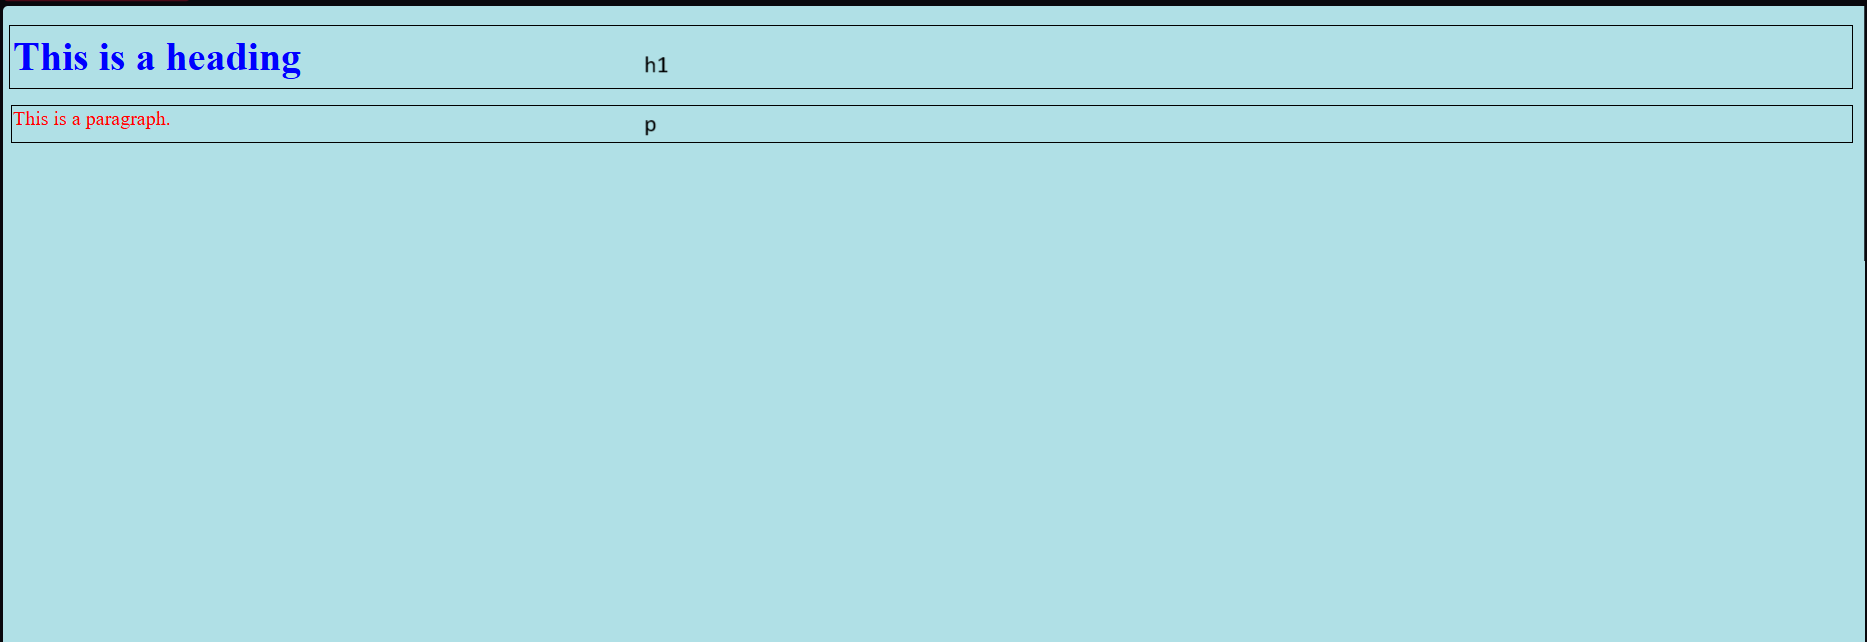
\includegraphics[scale=0.4]{Ex7.png}
\end{center}


\textbf{Ejemplo 8: External, Border} \\

HTML:

\lstinputlisting[language=html]{cssexternalex_border.html}


CSS:
\lstinputlisting{cssexternalstyles_border.css}


\begin{center}
    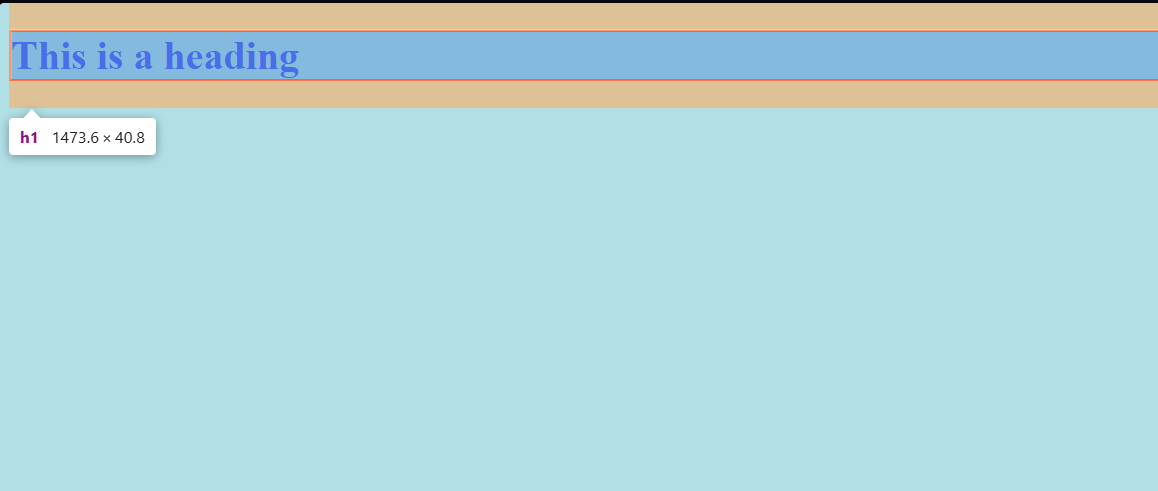
\includegraphics[scale=0.4]{Ex8.png}
\end{center}
\begin{center}
    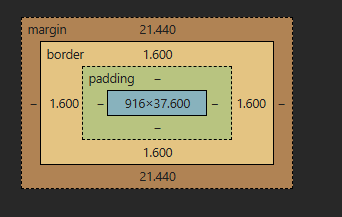
\includegraphics[scale=0.8]{Ex8bord.png}
\end{center}


\textbf{Ejemplo 9: External, Padding} \\

HTML:

\lstinputlisting[language=html]{cssexternalex_padding.html}


CSS:
\lstinputlisting{cssexternalstyles_padding.css}


\begin{center}
    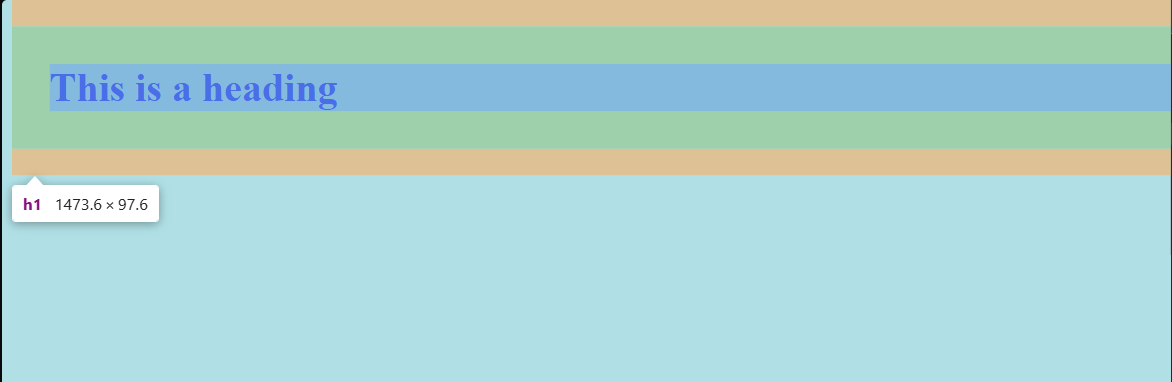
\includegraphics[scale=0.4]{Ex9.png}
\end{center}
\begin{center}
    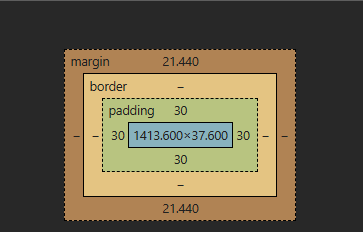
\includegraphics[scale=0.8]{Ex9bord.png}
\end{center}



\textbf{Ejemplo 9: External, Margin} \\

HTML:

\lstinputlisting[language=html]{cssexternalex_margin.html}


CSS:
\lstinputlisting{cssexternalstyles_margin.css}


\begin{center}
    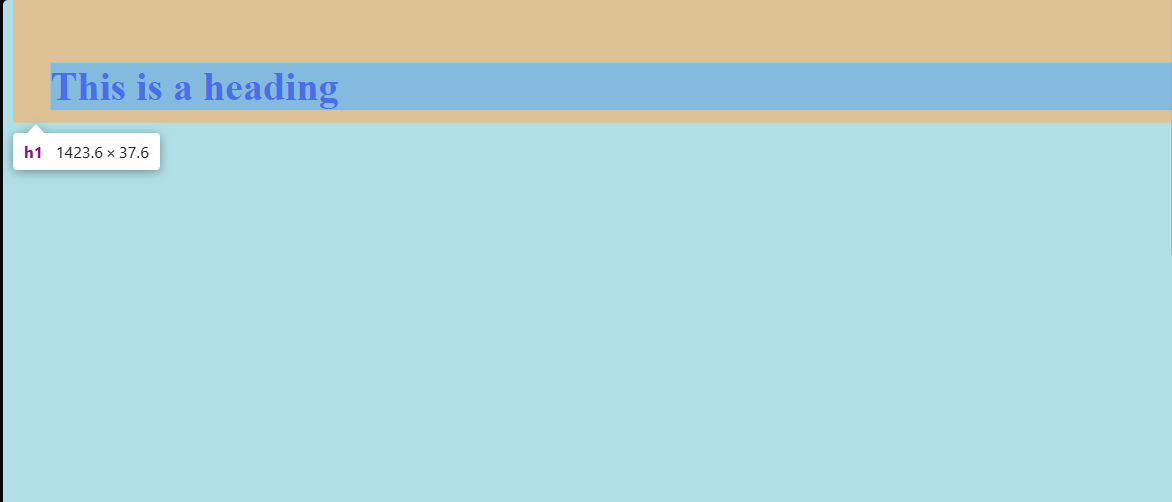
\includegraphics[scale=0.4]{Ex10.png}
\end{center}
\begin{center}
    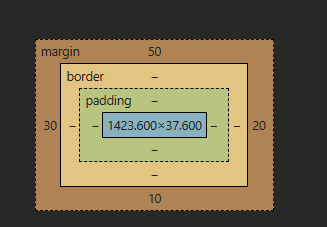
\includegraphics[scale=0.8]{Ex10bord.png}
\end{center}

\subsection{Actividad:}
Una presentación nuestra:

HTML:
\lstinputlisting[language=html]{presentacion.html}

CSS:
\lstinputlisting{presentacion.css}

\begin{center}
    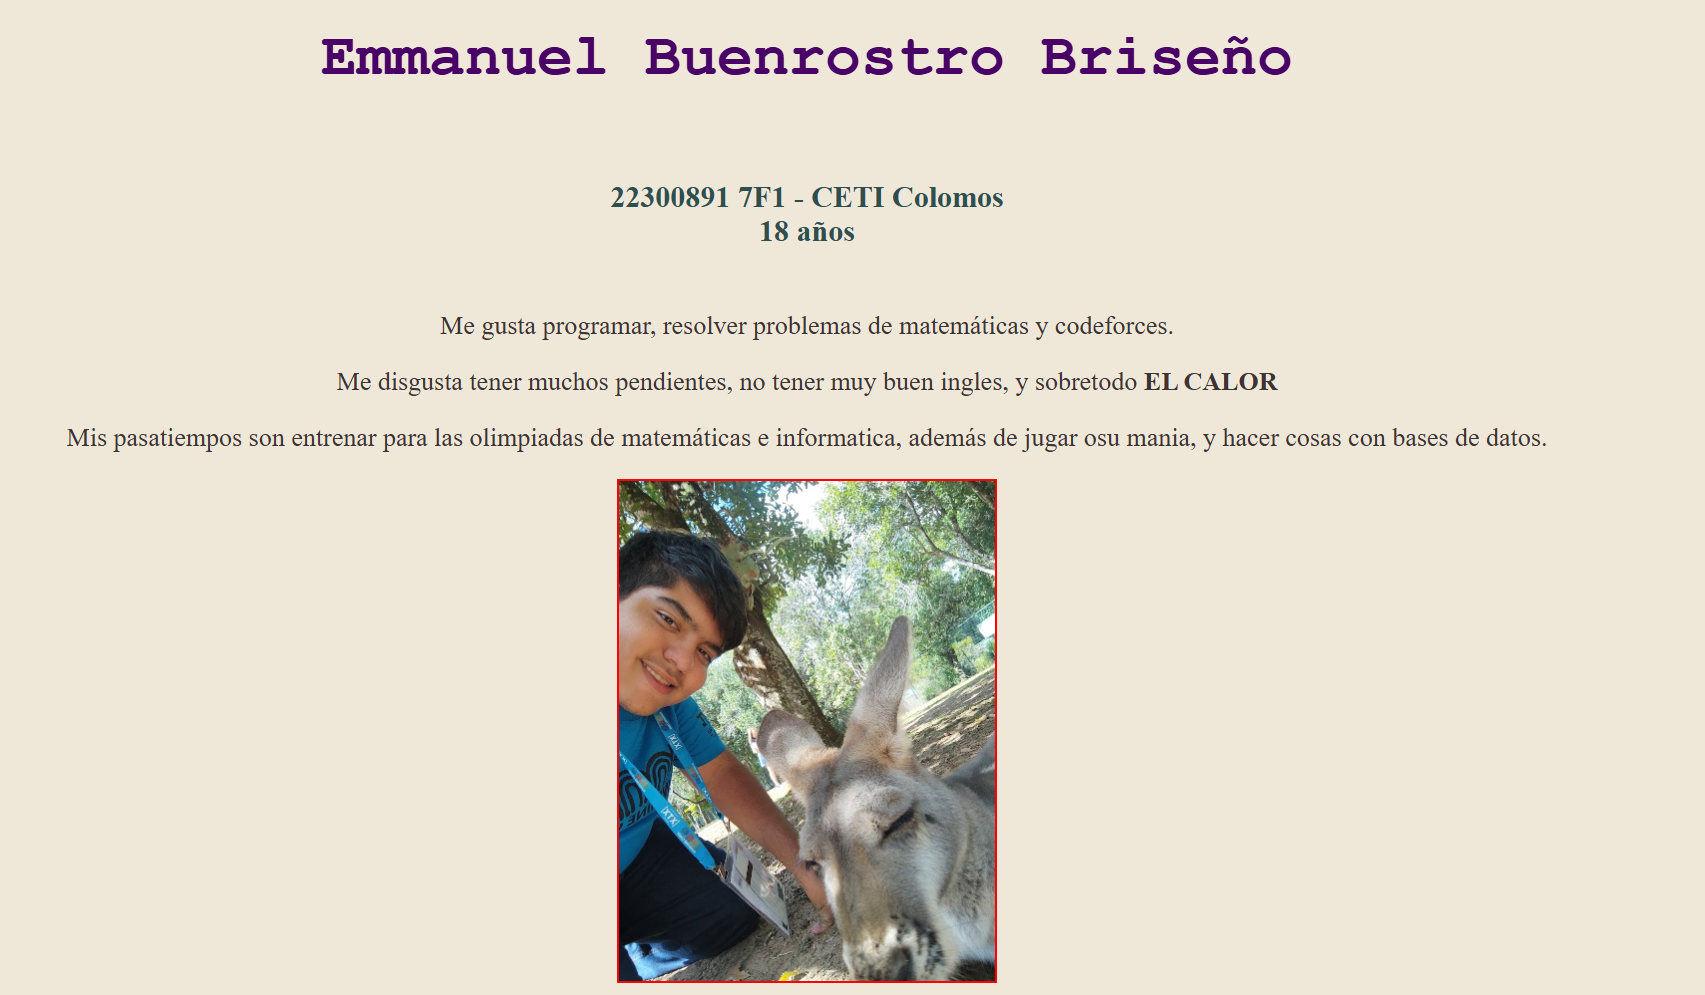
\includegraphics[scale=0.4]{Presentacionimg.png}
    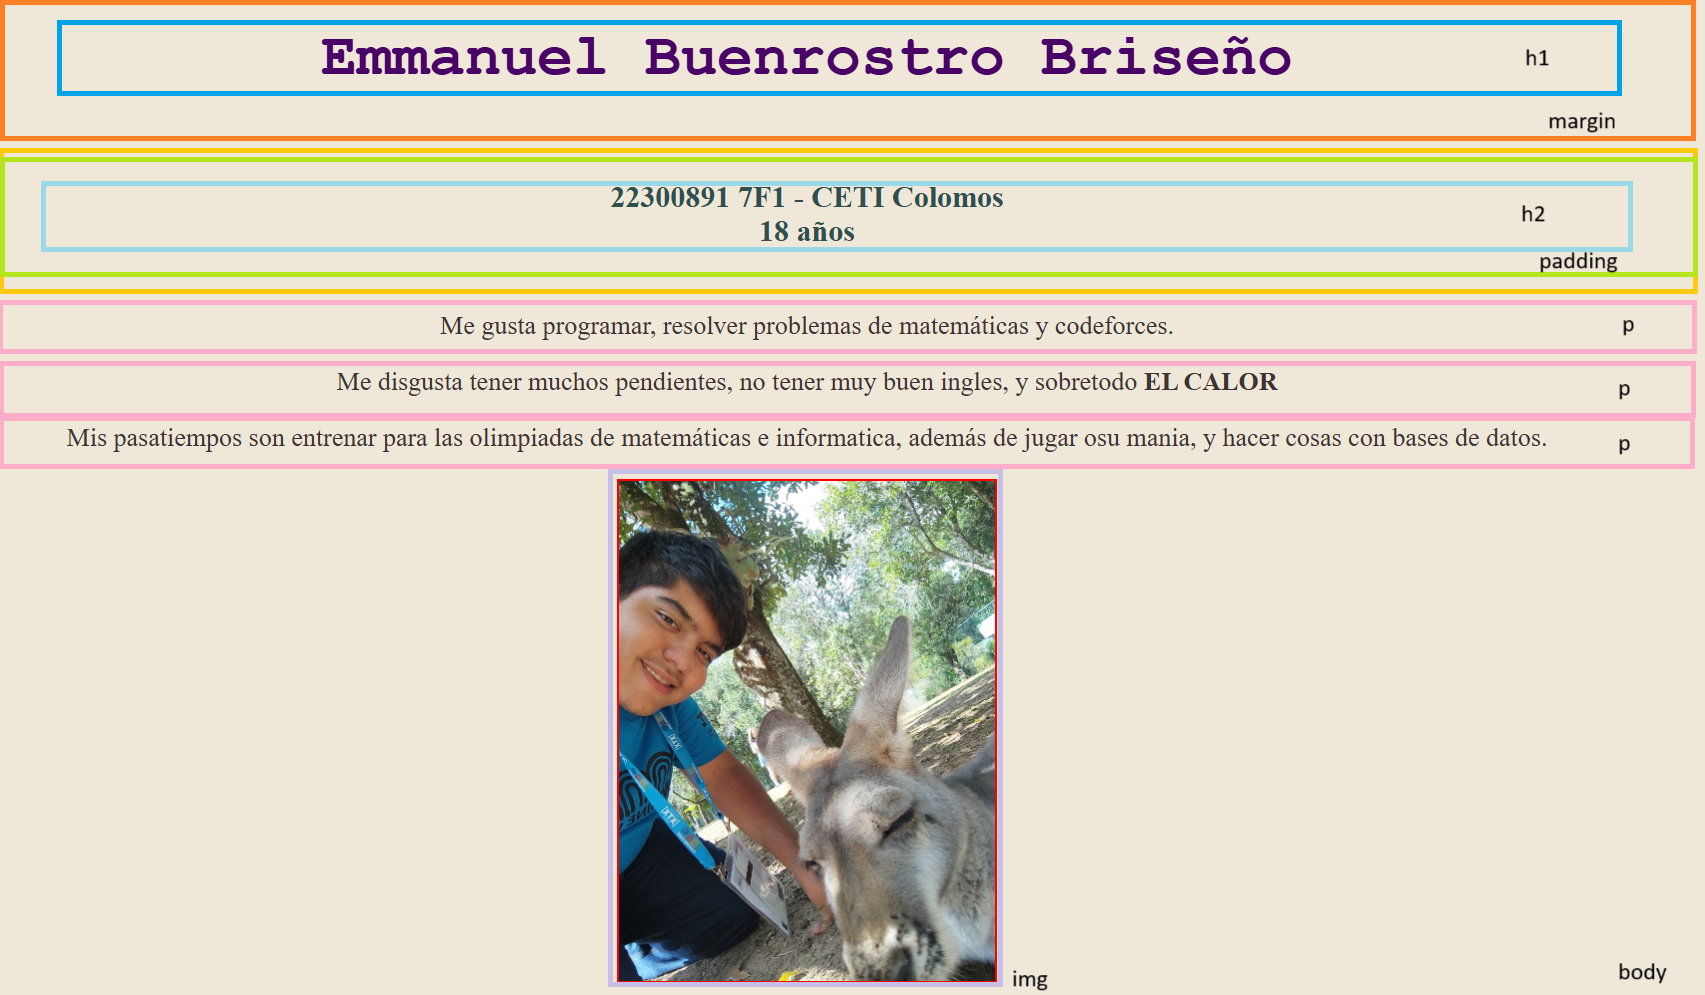
\includegraphics[scale=0.4]{presentacionpartes.png}
\end{center}




\section{Conclusión}

CSS probablemente es de lo que menos se usar en una pagina web, 
ya que la verdad no tengo mucha creatividad con el estilo, pero es muy util 
para hacer que la pagina web se vea mas usable para el usuario. 

    \section{Bibliografía}
\nocite{*}
\printbibliography[heading=bibintoc,title={.}]

    \end{document}